\documentclass[12pt,fleqn]{article}
\usepackage{
  amsmath,
  amssymb,
  booktabs,
  geometry,
  graphicx,
  microtype,
  parskip,
  caption,
}
\usepackage[shortlabels]{enumitem}

\geometry{margin=3cm}

% equation line spacing
\setlength{\jot}{0.5cm}

% meta data
\newcommand{\chapter}{6.1}
\newcommand{\authorname}{Amo DelBello}
\newcommand{\classdescription}{MATH 1350-D2}
\newcommand{\classname}{Introduction to Statistics, Fall 2022}
\newcommand{\assignment}{\chapter\ Book Assignment}

\newcommand{\problem}[1]{\vspace{5ex}\section*{\chapter-#1}}
\newcommand{\thead}[1]{\textnormal{\textbf{#1}}}
\newcommand{\tvspace}{\vspace{.25cm}}

\title{\classdescription\ \\ \classname\ \\ $\ $ \\ \assignment}
\author{\authorname}
\date{\today}


\begin{document}

\maketitle

(I used StatCrunch to calculate the answers for  problems 9\--12 and 41\--44.)
\problem{9}
0.6700

\problem{10}
0.8508


\problem{11}
$0.79954581 - 0.10027257 = 0.6993$


\problem{12}
$0.85769035 - 0.2514289 = 0.6063$


\problem{25}
\begin{figure}[ht]
  \centering
  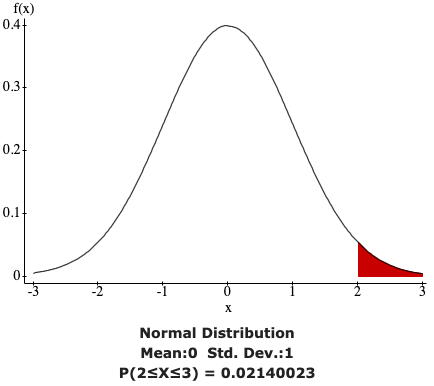
\includegraphics[width=8cm]{assets/25-bone-density.png}
  \caption*{$p(2 \le x \le 3) = 0.0214$}
\end{figure}


\problem{30}
\begin{figure}[ht]
  \centering
  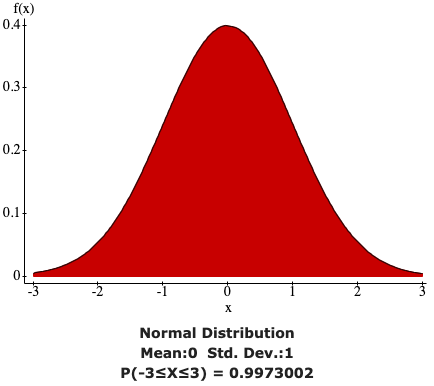
\includegraphics[width=8cm]{assets/30-bone-density.png}
  \caption*{$p(-3 \le x \le 3) = 0.9973$}
\end{figure}
\pagebreak


\problem{37}
\begin{figure}[ht]
  \centering
  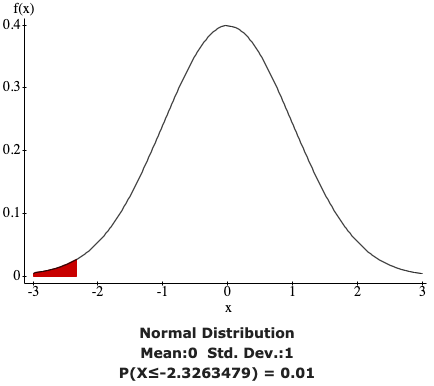
\includegraphics[width=8cm]{assets/37-bone-density.png}
  \caption*{$P_{99} = -2.33$}
\end{figure}


\problem{38}
\begin{figure}[ht]
  \centering
  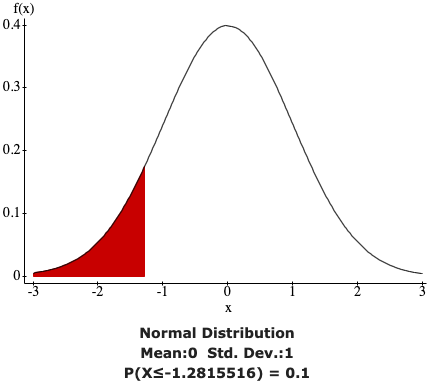
\includegraphics[width=8cm]{assets/38-bone-density.png}
  \caption*{$P_{10} = -1.28$}
\end{figure}
\pagebreak


\problem{39}
\begin{figure}[ht]
  \centering
  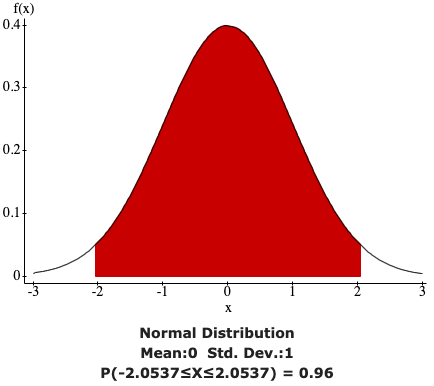
\includegraphics[width=8cm]{assets/39-bone-density.png}
  \caption*{Cutoff points: -2.05 and 2.05}
\end{figure}


\problem{40}
\begin{figure}[ht]
  \centering
  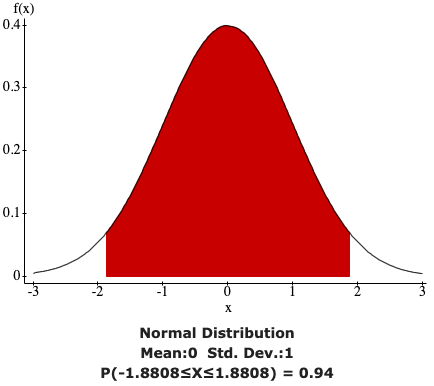
\includegraphics[width=8cm]{assets/40-bone-density.png}
  \caption*{Cutoff points: -1.88 and 1.88}
\end{figure}
\pagebreak


\problem{41}
Critical Value = 1.28


\problem{42}
Critical Value = 2.054


\problem{43}
Critical Value = 1.75


\problem{44}
Critical Value = 1.04


\end{document}
%%% Local Variables:
%%% mode: latex
%%% TeX-master: t
%%% End:
